
\ifprof
\else

\textbf{Vous trouverez à la fin de ce sujet une annexe contenant des informations concernant les programmes à écrire en 
\texttt{python}}
\fi

\section{Mise en situation}
\ifprof
\else
\vspace{.25cm}

\noindent \begin{minipage}[c]{.5\linewidth}
On étudie les transferts thermiques dans le mur d’une maison. La température à
l'intérieur de la maison est constante dans le temps et égale à $T_{\text{int}}=20^{\text{o}} \text{C}$. Aux temps 
négatifs $t<0$, la température extérieure est égale à $T_{\text{ext,1}}=10^{\text{o}} \text{C}$. À $t=0$, elle chute 
brusquement à $T_{\text{ext,2}}=-10^{\text{o}} C$ et elle reste égale à cette valeur aux temps positifs ($t>0$). On
souhaite étudier l'évolution du profil de température dans le mur au cours du temps.

Le mur a une épaisseur $e=40\;\text{cm}$. Les propriétés physiques du mur sont constantes : conductivité 
thermique$\lambda = 1,65\; \text{W.m}^{-1}.\text{K}^{-1}$, capacité thermique massique : $c_p = 1\, 000\; 
\text{J}.\text{kg}^{-1}.\text{K}^{-1}$, masse volumique : $\rho = 2\, 150 \; \text{kg}.\text{m}^{-3}$. 

\end{minipage} \hfill
\begin{minipage}[c]{.5\linewidth}
\begin{center}
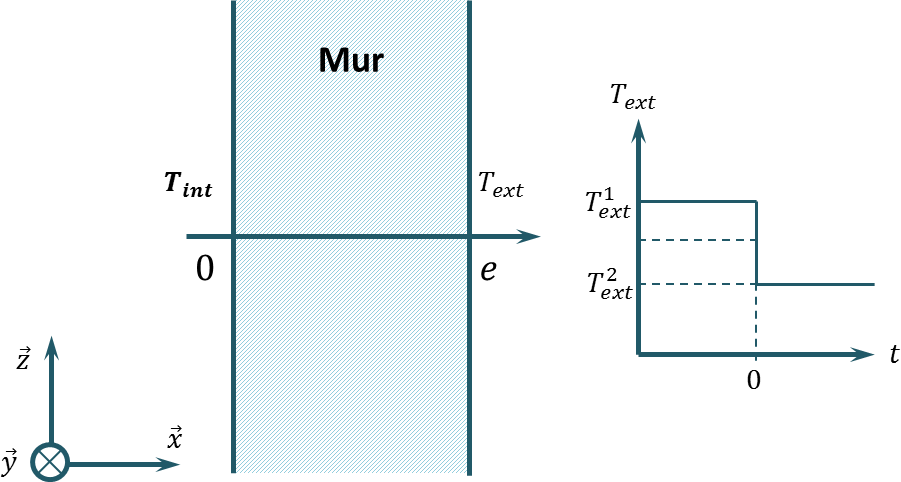
\includegraphics[width=\linewidth]{images/figure_01}
\end{center}
\end{minipage}

\noindent
On suppose que les longueurs $L_y$ et $L_z$ suivant $\vect{y}$ et $\vect{z}$ sont très grandes devant l'épaisseur $e$. 
En conséquence, on suppose que la température $T$ dans le mur ne dépend que du temps $t$ et de la coordonnée $x$. La 
coordonnée $x$ variera de 0 à $e$.

\begin{obj}
L'objectif est de déterminer l'évolution du flux thermique dans le mur au cours du temps. Pour cela, on s'appuiera sur 
la résolution d'une équation différentielle en utilisant un schéma explicite puis implicite.
\end{obj}
\fi

\subsection{Équation gouvernant la température}

\ifprof
\else

En l'absence de source d'énergie, l'équation régissant le transport de la chaleur s'exprime ainsi :
\begin{equation}
\mathbf{\rho c_p \dfrac{\partial T(x,y,z,t)}{\partial t} =  \lambda  \Delta T(x,y,z,t)}
\end{equation}
On rappelle la définition du Laplacien d'une fonction suffisamment régulière 
$\Delta f =\frac{\partial^2 f}{\partial x^2}+\frac{\partial^2 f}{\partial y^2}
+\frac{\partial^2 f}{\partial z^2}$.

\subparagraph{}\textit{En utilisant les hypothèses dimensionnelles, donner l'équation de la chaleur simplifiée. }

\fi

\ifprof
\begin{corrige}
\question\
$$ 
\rho c_p \dfrac{\partial T(x,t)}{\partial t} =  \lambda  \dfrac{\partial^2 T(x,t)}{\partial x^2}
$$
\end{corrige}
\else
\fi

\subsection{Conditions aux limites}

\ifprof
\else
On envisage  plusieurs types de conditions aux limites :
\begin{itemize}
\item \textbf{cas 1 : } la température est imposée aux limites du système;
\item \textbf{cas 2 : } la paroi extérieure est isolée par un matériau de très faible conductivité. 
\end{itemize}

\subparagraph{}\textit{Traduire chacune de ces conditions aux limites sur la fonction $T(x,t)$ et/ou sa dérivée.} 

\vspace{.5cm}

\textbf{Dans la suite, seul le premier cas sera étudié.}

\subparagraph{}\textit{Résoudre l'équation de la chaleur simplifiée \textbf{en régime permanent} dans les conditions suivantes : 
\begin{itemize}
\item \textbf{conditions 1 : } pour un instant particulier négatif $t_1<0$;
\item \textbf{conditions 2 : } pour un instant particulier positif  $t_2>0$, très longtemps après la variation de température extérieure quand le régime permanent est de nouveau établi dans le mur.
\end{itemize}
} 



\subparagraph{}\textit{Quelle est la nature des profils $T(x)$ obtenus (en régime permanent) à ces deux instants ? 
Tracer à la main les deux profils sur un même graphique sur la copie.}

\fi

\ifprof
\begin{corrige}
\question\
\begin{itemize}
\item \textbf{cas 1 : } $T(0,t)=T_{\text{int}}$ et $T(e,t)=T_{\text{ext}}$;
\item \textbf{cas 2 : } $T(0,t)=T_{\text{int}}$ et $ \dfrac{\partial T}{\partial t} (e,t)=0$.\\
\end{itemize}

\question\
En régime permanent, l'équation différentielle devient : $\dfrac{\partial^2 T(x,t)}{\partial x^2}=0$. On a donc :
$T(x) =  k_1 x + k_2 $. Par suite : $T(0)=T_{\text{int}}=k_2$ et $T(e)=T_{\text{ext}} = k_1 e + k_2 $. On a donc : 
$ k_1 =\dfrac{T_{\text{ext}} -T_{\text{int}}}{e} $. Au final : $T(x) =  \dfrac{T_{\text{ext}} -T_{\text{int}}}{e} x + 
T_{\text{int}} $.

\begin{itemize}
\item \textbf{conditions 1 : } lorsque $t_1 <0$,  $T_{\text{int}}=20^{\text{o}} \text{C}$ et 
$T_{\text{ext,1}}=10^{\text{o}} \text{C}$. En conséquence, $T(x) =  \dfrac{T_{\text{ext,1}} -T_{\text{int}}}{e} x + 
T_{\text{int}} $.
\item \textbf{conditions 2 : }  lorsque $t_2 >0$,  $T_{\text{int}}=20^{\text{o}} \text{C}$ et 
$T_{\text{ext,2}}=-10^{\text{o}} \text{C}$. En conséquence, $T(x) =  \dfrac{T_{\text{ext,2}} -T_{\text{int}}}{e} x + 
T_{\text{int}} $.\\
\end{itemize}


\question\

\begin{center}
	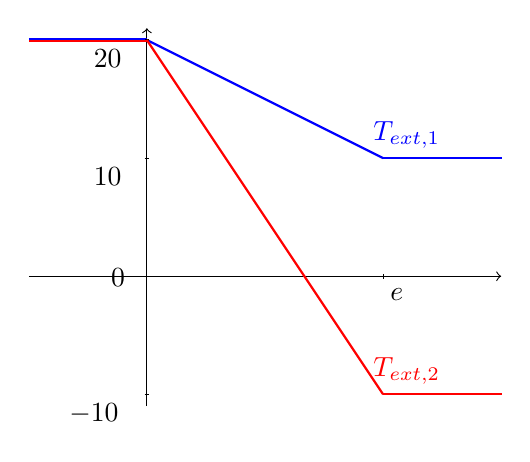
\begin{tikzpicture}[scale = 0.15]
	  \draw[->] (-10,0) -- (30,0);
	  \draw[->] (0,-11) -- (0,21);
	 % \clip (-0.3,-0.3) rectangle (pi+0.2,0.7);
	  \draw[domain=(-10):(0),samples=200,smooth,variable=\x,blue,thick] 
plot({\x},{20+0.1});
	  \draw[domain=(0):(20),samples=200,smooth,variable=\x,blue,thick] 
plot({\x},{-0.5*\x+20});
	  \draw[domain=(20):(30),samples=200,smooth,variable=\x,blue,thick] 
plot({\x},{10});
	  \draw[blue,thick] (22,12) node {$T_{ext,1}$};
	  \draw (20,0.2) -- (20,-0.2) node[anchor=north] {$~~~e$};
	  \draw (-0.1,-0.1) node {$0~~~~~~$};
	  \draw (-0.2,20) -- (0.2,20) node[anchor=north] {$20~~~~~~~~~$};
	  \draw (-0.2,10) -- (0.2,10) node[anchor=north] {$10~~~~~~~~~$};
	  \draw (-0.2,-10) -- (0.2,-10) node[anchor=north] {$-10~~~~~~~~~~~~$};
	  \draw[domain=(-10):(0),samples=200,smooth,variable=\x,red,thick] 
plot({\x},{20-0.1});
	  \draw[domain=(0):(20),samples=200,smooth,variable=\x,red,thick] 
plot({\x},{-1.5*\x+20});
	  \draw[domain=(20):(30),samples=200,smooth,variable=\x,red,thick] 
plot({\x},{-10});
	  \draw[red,thick] (22,-8) node {$T_{ext,2}$};
	  
	\end{tikzpicture}
        %\caption{Courbe représentant $f$.}
\end{center}

\end{corrige}
\else
\fi

\section{Résolution numérique : méthode des différences finies}

\ifprof
\else
On cherche à résoudre numériquement l'équation aux dérivées partielles : 
\begin{equation}
\mathbf{\alpha \dfrac{\partial T(x,t)}{\partial t} = \dfrac{\partial^2 T(x,t)}{\partial x^2}} \quad \text{avec }\alpha \text{ constante.}
\end{equation}
Les conditions aux limites sont les suivantes :
\begin{itemize}
\item $T(0,t)=T_{\text{int}}$ pour $t>0$;
\item $T(e,t)=T_{\text{ext,2}}$ pour $t>0$;
\item $T(x,0)=ax + b$ pour $x\in[0,e]$.
\end{itemize}

\subparagraph{}\textit{Quelle est l'expression de $\alpha$ en fonction des paramètres physiques du mur ?}


\subparagraph{\label{q_tini}}\textit{Exprimer $a$ et $b$ en fonction de $T_{\text{int}}$,$T_{\text{ext,1}}$ et $e$.}
\fi

\ifprof
\begin{corrige}
\question\
On a $\alpha =\dfrac{\rho c_p}{\lambda}$.\\

\question\
On a, pour t<0, $T(0,0)= b = T_{\text{int}}$ et  $T(e,0)= ae+ T_{\text{int}}= T_{\text{ext,1}}$. On a donc : $a= \dfrac{T_{\text{ext,1}}- T_{\text{int}}}{e}$. Au final :
$$T(x,0)=\dfrac{T_{\text{ext,1}}- T_{\text{int}}}{e} x + T_{\text{int}} \quad \text{pour } x\in[0,e].$$
\end{corrige}
\else
\vspace{.5cm}

La partie suivante permettra de déterminer une solution de l'équation aux dérivées partielles en utilisant la méthode des différences finies.

\fi

\subsection{Discrétisation dans l'espace et dans le temps}

\ifprof
\else

\noindent \begin{minipage}[c]{.6\linewidth}
On divise l'intervalle $[0,e]$, représentant l'épaisseur du mur, en $N+2$ points, numérotés de 0 à $N+1$, régulièrement 
espacés de $\Delta x$. Cette division est appelée << discrétisation >>. La distance $\Delta x$ est appelée le << pas 
d’espace >>. A l'intérieur du mur (frontières intérieure et extérieure exclues) se trouvent donc $N$ points. On cherche 
à obtenir la température en ces points particuliers à chaque instant. 


\end{minipage} \hfill
\begin{minipage}[c]{.38\linewidth}
\begin{center}
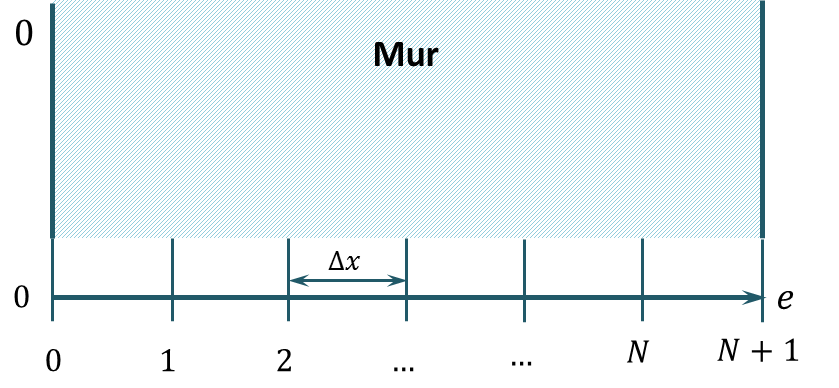
\includegraphics[width=\linewidth]{images/figure_02}
\end{center}
\end{minipage}

\subparagraph{\label{q_xini}}\textit{Donner l'expression de $\Delta x$ en fonction de $N$ et de l'épaisseur du mur $e$.}



\subparagraph{\label{q_xini2}}\textit{Donner l'abscisse $x_i$ du i\ieme point 
en fonction de $i$ et $\Delta x$, sachant que $x_0=0$ et  $x_{N+1} = e$.}

\fi

\ifprof
\begin{corrige}
\question\
On a : $\Delta x = \dfrac{e}{N+1}$.\\

\question\
On a : $x_i = i \Delta x$.
\end{corrige}
\else

\vspace{.5cm}

Le temps est discrétisé en \textit{ItMax} intervalles de durée $\Delta t$ et on ne s'intéresse 
au profil de température qu'aux instants particuliers $t_k = k \cdot \Delta t$. 
L'intervalle élémentaire de temps $\Delta t$ est appelé le << pas de temps >>.

\noindent
Deux méthodes de résolutions sont proposées : 
\begin{itemize}
\item méthode utilisant un schéma explicite;
\item méthode utilisant un schéma implicite.
\end{itemize}
\fi

\subsection{Méthode utilisant un schéma explicite}

\ifprof
\else
\begin{obj}
Déterminer le schéma explicite permettant la résolution de l'équation de la chaleur.
\end{obj}

On donne le développement limité à l'ordre 3 de $T(x+\Delta x,t)$ et $T(x-\Delta x,t)$ :
$$
T(x+\Delta x,t)=T(x,t)+\dfrac{\partial T(x,t)}{\partial x}\Delta x 
+ \dfrac{1}{2}\dfrac{\partial^2 T(x,t)}{\partial x^2} \;\left( \Delta x\right)^2 
+ \dfrac{1}{6}\dfrac{\partial^3 T(x,t)}{\partial x^3} \;\left( \Delta x\right)^3 
+ o\left( \Delta x^3\right)
$$

$$
T(x-\Delta x,t)=T(x,t)-\dfrac{\partial T(x,t)}{\partial x}\Delta x 
+ \dfrac{1}{2}\dfrac{\partial^2 T(x,t)}{\partial x^2} \;\left( \Delta x\right)^2 
- \dfrac{1}{6}\dfrac{\partial^3 T(x,t)}{\partial x^3}\;\left( \Delta x\right)^3 
+ o\left( \Delta x^3\right)
$$

\subparagraph{}\textit{En déduire une expression approchée à l'ordre 1 de
 $\left[\dfrac{\partial^2 T(x,t)}{\partial x^2}\right]_{x,t}$ (dérivée partielle spatiale seconde de 
 $T$ évaluée au point $x$ à l'instant $t$) en fonction de $T(x+\Delta x,t)$, $T(x-\Delta x,t)$ et 
$T(x,t)$ et $\Delta x$.}



\vspace{.5cm}

On note $T_i^k$ la température $T\left(x_i,t_k\right)$, évaluée au point d'abscisse $x_i$ à
 l'instant $t_k$. De même, on note $T_{i+1}^k=T\left(x_i + \Delta x,t_k \right)$ et 
$T_{i-1}^k=T\left(x_i - \Delta x,t_k \right)$.

\subparagraph{}\textit{Déduire de la question précédente que  
$\left[\dfrac{\partial^2 T(x,t)}{\partial x^2}\right]_{x_i,t_k} \approx
\dfrac{T_{i+1}^k-2T_{i}^k + T_{i-1}^k}{\Delta x^2 } $ (dérivée partielle seconde de 
$T$ évaluée en $x_i$ à l'instant $t_k$).}


\vspace{0.5cm}
La dérivée partielle temporelle de l'équation différentielle est maintenant approchée grâce à un
développement limité.

En utilisant le même raisonnement en réalisant un développement limité de la fonction 
$t\mapsto T(x,t)$ à l'ordre $1$, on obtiendrait l'équation suivante valable en chaque point
 d'abscisse $x_i$ et à chaque instant $t_k$ : 
$$
\left[\dfrac{\partial T(x,t)}{\partial t}\right]_{x_i,t_k} 
=
\dfrac{T_{i}^{k+1}- T_{i}^k}{\Delta t }.
$$



\subparagraph{}\textit{En utilisant les questions précédentes, montrer que 
l'équation différentielle peut se mettre sous la forme : 
$$
T_{i}^{k+1} = r T_{i-1}^{k} + \left( 1-2r \right) T_i^k + r T_{i+1}^k.
$$ 
}
$r$ sera explicité en fonction de $\Delta x$, $\Delta t$ et $\alpha$.

\vspace{.5cm}

Dans toute la suite on considère que l'on a défini $r$ et que l'on peut l'utiliser directement. 
\vspace{.5cm}

L'équation précédente est appelée schéma numérique explicite. Si on connaît la température en tous les points 
$x_1$, $x_2$, ..., $x_N$ à  l'instant $t_k$ on peut calculer grâce à elle la température en tous les points à l'instant 
$t_{k+1}$.

\subparagraph{}\textit{L'équation est-elle valable dans tout le domaine, c'est-à-dire pour toute valeur de $i$, $0\leq 
i\leq N+1$ ? Que valent $T_0^k$ et $T_{N+1}^k$ ?}

\subparagraph{}\textit{Montrer que pour tout instant $k$, le problème peut se mettre sous la forme matricielle suivante : }
$$
T^{k+1} = M \cdot T^k + rV \quad \text{avec} \quad T^k =
 \begin{pmatrix} T_1^k \\  T_2 ^k \\ ... \\  T_{N-1}^{k} \\ T_{N}^{k}  \end{pmatrix}.
$$
\textit{avec M une matrice carrée $N\times N$, $V$ un vecteur de taille $N$ que l'on explicitera.}


%\subparagraph{}
%\textit{Donner toutes les composantes de $T^0$.}
%\begin{corrige}
%\end{corrige}
%\ifprof
%\else
%\fi

\vspace{.5cm}
Ainsi, à chaque pas de temps $k$, on calculera un vecteur $T^k$ contenant la température à chaque abscisse $i$ du mur.

\begin{center}
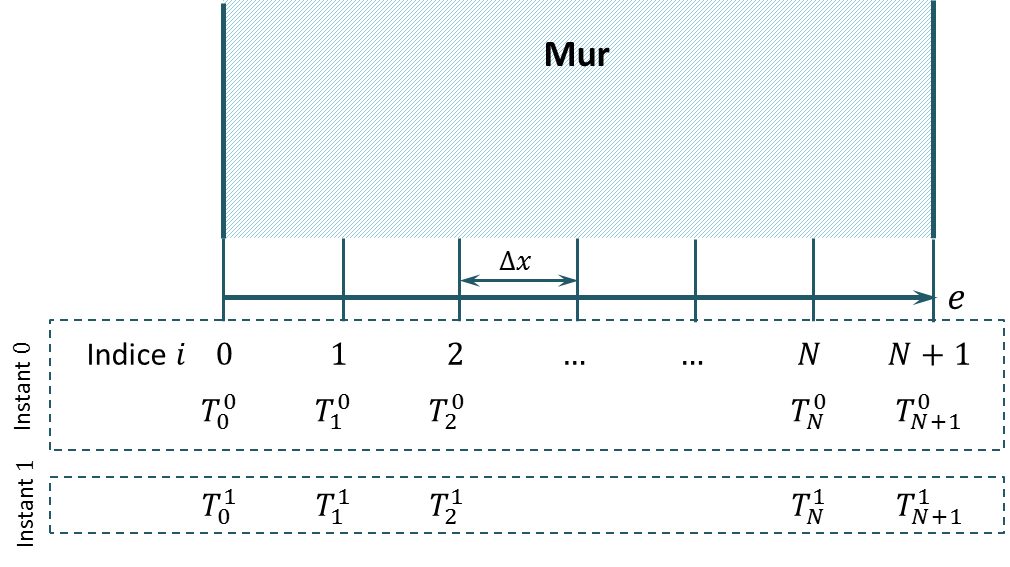
\includegraphics[width=0.5\linewidth]{images/figure_03}
\end{center}

\subparagraph{}
\textit{Expliciter succinctement comment déterminer la température dans le mur à chaque instant.}



\vspace{.5cm}

\noindent
Une annexe est fournie en fin de sujet vous rappelant quelques fonction de la bibliothèque \textbf{Numpy}.

\subparagraph{}
\textit{On donne \texttt{ T0} le vecteur température à l'instant $k=0$. 
Écrire la fonction \texttt{euler\_explicite(M,T0,V,k)} retournant le vecteur de température 
$T^k$ à l'instant $k$. Cette fonction sera définie de manière \textbf{récursive}.}\\
\fi

\ifprof
\begin{corrige}\question\
On additionne les deux lignes, on a directement :
$$
T(x+\Delta x,t)+T(x-\Delta x,t)=2T(x,t)
+ \dfrac{\partial^2 T(x,t)}{\partial x^2}(\Delta x)^2
+o((\Delta x)^3)$$
puis on isole : 
$$
\dfrac{\partial^2 T(x,t)}{\partial x^2} 
=
\dfrac{T(x+\Delta x,t)-2T(x,t) + T(x-\Delta x,t)}{\Delta x^2 }+ o\left(\Delta x\right)
$$



\question\
$$
\left[\dfrac{\partial^2 T(x,t)}{\partial x^2}\right]_{x_i,t_k} 
=
\dfrac{T_{i+1}^k-2T_{i}^k + T_{i-1}^k}{\Delta x^2 }
$$

\question\
En injectant les approximations dans l'EDP, nous obtenons $T^{k+1}_{i}-T_i^k=\dfrac{\Delta t}{\alpha\Delta 
x^2}\p{T_{i+1}^k-2T_i^k+T_{i-1}^k}$. Ainsi,
$r=\dfrac{\Delta t}{\alpha \Delta x^2}$\\

\question\ Pas pour $i=0$ et $i=N+1$. Pour ces valeurs nous avons : $T_0^k = 20^o C$ et $T^k_{N+1}=-10^o C$. \\

\question\
On a, pour $i\in \left]0;N+1 \right[$ :
$$
\begin{array}{ll}
i & T_{i}^{k+1} = r T_{i-1}^{k} + \left( 1-2r \right) T_i^k + r T_{i+1}^k \\
\hline 
\hline 
\\
%T_{0}^{k+1} = r T_{0-1}^{k} + \left( 1-2r \right) T_i^k + r T_{0+1}^k \\
i=1 & T_{1}^{k+1} = r T_{0}^{k} + \left( 1-2r \right) T_1^k + r T_{2}^k \\
i=2 & T_{2}^{k+1} = r T_{1}^{k} + \left( 1-2r \right) T_2^k + r T_{3}^k \\
i=3 & T_{3}^{k+1} = r T_{2}^{k} + \left( 1-2r \right) T_3^k + r T_{4}^k \\
&\\
i=N -1& T_{N -1}^{k+1} = r T_{N -2}^{k} + \left( 1-2r \right) T_{N -1}^k + r T_{N}^k \\
i=N & T_{N}^{k+1} = r T_{N-1}^{k} + \left( 1-2r \right) T_N^k + r T_{N+1}^k \\
\end{array}
$$ 

On a donc : 
$$
T^{k+1} = M \cdot T^k + rV
$$
avec :
$$
M = 
\begin{pmatrix}
1-2r & r     & 0 & 0 & 0 &  \ldots & 0 \\
r     & 1-2r & r & 0 & 0  & \ldots &  0 \\
0    & r & 1-2r & r & 0   & \ldots&  0 \\
\vdots & \vdots & \vdots & \vdots & \vdots & \ldots & \ldots \\
0& 0& 0& 0& 0& r & 1-2r\\
\end{pmatrix}
\quad \text{et} \quad 
V = \begin{pmatrix}
T_0^k = T_{\text{int}} \\
0 \\
\vdots \\
0 \\
T_N^k = T_{\text{ext,2}} \\
\end{pmatrix}.
$$

\question\
\`A l'instant $t=0$, le flux de température dans le mur est connu. La température extérieure passe alors à $-10^o C$. On 
utilise alors l'équation de récurrence.

(Lors du codage de la méthode explicite, il faut faire attention à la divergence du schéma. Pour cela, il faut prendre 
des intervalles de temps << petits >>.)\\

\question\
\begin{python}
def euler_explicite(M,T_0,r,V,k):
    if k==0:
        return T_0
    else:
        T=euler_explicite(M,T_0,r,V,k-1)
        return numpy.dot(M,T)+r*V
        
\end{python}
\end{corrige}
\else
\fi




\subsection{Méthode utilisant un schéma implicite}

\ifprof
\else
\begin{obj}
Déterminer une méthode permettant de résoudre l'équation de la chaleur à partir du 
schéma implicite donné.
\end{obj}

En utilisant un schéma d'Euler implicite, on montre que l'équation 
$\alpha \dfrac{\partial T(x,t)}{\partial t} = \dfrac{\partial^2 T(x,t)}{\partial x^2}$
 peut se mettre sous la forme suivante : 
$$
T_i^k = -rT_{i-1}^{k+1} + \left( 1+2r\right) T_{i}^{k+1}-rT_{i+1}^{k+1}.
$$

La température à l'instant $t_k$ est exprimée en fonction de la température à l'instant 
ultérieur $t_{k+1}$.
Le système d'équation peut être écrit sous la forme matricielle : 
\begin{equation} \label{eq_implicite}
\mathbf{M T^{k+1} = T^k + rV}.
\end{equation}
avec : 

$$
M = 
\begin{pmatrix}
1+2r & -r     & 0 & 0 & 0 &  \ldots & 0 \\
-r     & 1+2r & -r & 0 & 0  & \ldots &  0 \\
0    & -r & 1+2r & -r & 0   & \ldots&  0 \\
\vdots & \vdots & \vdots & \vdots & \vdots & \ldots & \ldots \\
0& 0& 0& 0& 0& -r & 1+2r\\
\end{pmatrix}
\quad 
V = \begin{pmatrix}
T_{\text{int}} \\
0 \\
\vdots \\
0 \\
T_{\text{ext}} \\
\end{pmatrix}
\quad 
T^k = \begin{pmatrix}
T_1^k \\
T_2^k  \\
\vdots \\
T_{N-1}^k  \\
T_N^k \\
\end{pmatrix}.
$$



\subparagraph{}
\textit{Pour obtenir $T^{k+1}$ en fonction de $T^{k}$, il est nécessaire d'inverser le 
système matriciel à chaque pas de temps.
Donner le nom d'un algorithme permettant de faire cela et donner sa complexité.}


\begin{obj}
La matrice $M$ étant particulière (tridiagonale) , nous allons utiliser un algorithme plus 
performant pour résoudre ce système matriciel tridiagonal : l'algorithme de Thomas.
 Le système que l'on cherche à résoudre est le suivant : 
$$
M U = D 
$$
$M$ est une matrice tridiagonale de dimension $N\times N$, c'est à dire que tous les éléments 
sont nuls sauf les diagonales principales, supérieures et inférieures. 
\end{obj}

On a donc : 
$$
M = 
\begin{pmatrix}
b_0 & c_0 &  &  &  &  & \\
a_1 & b_1 & c_1 & &0 & &\\
      & a_2 & b_2 & c_2 & & & \\
& & \ddots & \ddots & \ddots & \\
& 0& & a_{N-2} & b_{N-2} & c_{N-2}\\
& & & & a_{N-1} & b_{N-1}\\
\end{pmatrix}
\quad 
U = \begin{pmatrix}
u_0 \\
\vdots \\
\vdots \\
\vdots  \\
u_{N-1} \\
\end{pmatrix}
\quad 
D = \begin{pmatrix}
d_0 \\
\vdots \\
\vdots \\
\vdots  \\
d_{N-1} \\
\end{pmatrix}.
$$

Dans cet algorithme, on calcule les coefficients suivants : 
$$
c'_0 = \dfrac{c_0}{b_0} \quad c'_i = \dfrac{c_i}{b_i - a_i c'_{i-1}}  \quad \text{pour} \quad i=1,2,\ldots, N-2.$$

$$
d'_0 = \dfrac{d_0}{b_0} \quad d'_i = \dfrac{d_i-a_i d'_{i-1}}{b_i - a_i c'_{i-1}}  \quad \text{pour} \quad i=1,2,\ldots, 
N-1.
$$

Les inconnues $u_0, u_1, \ldots, u_{N-1}$ sont alors obtenues par les formules :
$$
u_{N-1} = d'_{N-1} \quad u_i = d'_i -c'_i u_{i+1} \quad  \text{pour} \quad i=N-2, N-3, \ldots, 1, 0.
$$


\subparagraph{}
\textit{En utilisant l'algorithme de Thomas, écrire une fonction \texttt{CalcTkp1(M,D)} 
qui retourne le vecteur $U$, solution du système matriciel, à partir de la matrice 
$M$ et du vecteur $D$.}\\

On pourra commencer par créer  des vecteurs contenant des zéros :
 A, B, C, Cp ,Dp (pour C' et D') et U.\\
 Puis on pourra  définir A, B et C à partir de la matrice $M$ et ensuite calculer Cp et Dp puis U.


\subparagraph{}
\textit{Donner la complexité de l'algorithme et comparer à celui de la question 16. 
On prendra en compte uniquement les tests, les affectations (même de tableaux)
 et les opérations élémentaires (+, -, *, /) qui compte chacune pour << un >>.}\\
\fi

\ifprof
\begin{corrige}\question\
On peut utiliser l'algorithme du pivot de Gauss. Sa complexité est en $\mathcal{O}(n^3)$.\\

\question\
Proposition de corrigé qui ne correspond pas exactement aux préconisations de l'énoncé :

\begin{python}
def CalcTkp1(M,D):
    N=D.shape[0]
    Cp=[M[0,1]/M[0,0]]
    Dp=[D[0,0]/M[0,0]]
    U=numpy.zeros((N,1))
    for i in range(1,N-1):
        Cp.append(M[i,i+1]/(M[i,i]-M[i,i-1]*Cp[i-1]))
        Dp.append((D[i,0]-M[i,i-1]*Dp[-1])/(M[i,i]-M[i,i-1]*Cp[i-1]))
    Dp.append((d[N-1,0]-M[N-1,N-2]*Dp[-1])/(M[N-1,N-1]-M[N-1,N-2]*Cp[-1]))
    U[N-1,0]=Dp[-1]
    for j in range(2,N):
        U[N-j,0]=Dp[N-j]-Cp[N-j]*U[N-j+1,0]
    return U
\end{python}

\question\
Cet algorithme contient deux boucles \texttt{for} indépendantes. Dans chacune de ces boucles, le nombre d'opérations 
est une constante. En dehors de ces boucles, il n'y a aussi que des opérations en temps constant. Ainsi la complexité 
de l'algorithme est linéaire (à comparer à une complexité cubique pour l'algorithme de Gauss).
\end{corrige}
\else
\fi


\section{Résolution de l'équation différentielle implicite}

\ifprof
\else
L'objectif est de calculer la température en chaque point au cours du temps. Parmi les variables
d'entrée se trouvera un vecteur $T_0$ de dimension $N$, défini en dehors de la fonction,
 contenant les valeurs de la température aux points de discrétisation à l'instant initial. 
 Au sein de la fonction, un algorithme calculera itérativement la température avec un 
 nombre maximal d'itérations ItMax. En sortie de la fonction, on récupérera le nombre 
 d'itérations réellement effectuées, \texttt{nbIter} et une matrice \texttt{T\_tous\_k}, de
  dimensions $N\times Itmax$.  Chaque colonne de cette matrice contient le vecteur $T^k$
   dont les éléments sont les valeurs de la température aux $N$ points $x_1$, ..., $x_N$, 
 points à l'intérieur du mur à l'instant $k$ :
$$
T^k = \begin{pmatrix} T_1^k \\  T_2 ^k \\ ... \\  T_{N-1}^{k} \\ T_{N}^{k}  \end{pmatrix}
\quad
T\_tous\_k = 
\begin{pmatrix} 
T_1^1   & T_1^2  & \cdots & T_1^{ItMax-1} & T_{1}^{ItMax} \vspace{0.3cm} \\
T_2^1   & T_2^2  & \cdots & T_2^{ItMax-1} & T_2^{ItMax }  \vspace{0.15cm}\\
\vdots & \vdots & \cdots & \vdots & \vdots \vspace{0.15cm}\\
T_{N-1}^1   & T_{N-1}^2  & \cdots & T_{N-1}^{ItMax-1} & T_{N-1}^{ItMax} \vspace{0.3cm} \\
T_{N}^1   & T_{N}^2  & \cdots & T_{N}^{ItMax-1} & T_{N}^{ItMax}  \\
 \end{pmatrix}.
$$


On souhaite arrêter le calcul lorsque la température ne varie presque plus dans le temps. 
Dans ce but, on évaluera la norme  de $T^k - T^{k-1}$ à chaque itération. 
\begin{defi}
On définit la norme d'un vecteur $v$ par : 
$$
||v|| = \sqrt{\sum\limits_{i=1}^{N}v_i^2} \quad \text{avec} \quad v=
\begin{pmatrix} v_1 \\ v_2 \\ \vdots \\ \vdots \\ v_n \end{pmatrix}.
$$
\end{defi}


\subparagraph{}
\textit{Écrire une fonction \texttt{calc\_norme} qui calcule la norme d'un vecteur. }


%\subparagraph{\label{q_solve}}
%\textit{Écrire \textbf{l'en-tête} de la fonction \texttt{schema\_implicite} permettant de calculer la température en 
%chaque point au cours du temps. Vous préciserez clairement les paramètres d'entrée et de sortie.}
\subparagraph{\label{q_solve}}
\textit{Écrire la fonction \texttt{solution(M,T,V)}, d'arguments une matrice $M$
 tridiagonale et deux vecteurs $T$ et $V$ et retournant le vecteur $U$ tels que $MU=T+rV$.}
 On utilisera la fonction \texttt{CalcTkp1}.


\subparagraph{}
\textit{Affecter la valeur 2000 à  \texttt{ ItMax}. Créer la matrice  \texttt{T\_tous\_k}  de dimensions $N\times 
ItMax$ en la remplissant de zéros.}

\subparagraph{}
\textit{D'après les questions précédentes la température $T$ dans le mur vérifie la condition
 initiale  $T(x,0)=ax+b$ où 
 $a=\dfrac{T_{\text{ext},1}-T_{\text{int}}}{e}$  et  $b=T_{\text{int}}$.\\
Écrire la fonction \texttt{T0(Tint,Text,N) } d'arguments la température intérieure $T_{\text{int}}$, 
la température extérieure $T_{\text{ext}}$ et l'entier $N$ et retournant le vecteur $T^0$, de taille $N$,
contenant les températures en chaque point du mur lorsque $t=0$. }
%\textit{En utilisant les résultats des questions \ref{q_tini}, \ref{q_xini} et \ref{q_xini2}, 
%écrire la fonction T0(Tint,Text,N) d'arguments la température intérieure $Tint$, 
%la température extérieure $Text$ et l'entier $N$ et retournant le vecteur $T^0$, de taille $N$,
%contenant les températures en chaque point du mur lorsque $t\leq 0$. }


\subparagraph{}
\textit{Écrire la suite d'instructions qui affecte à la première colonne de \texttt{T\_tous\_k} 
 le vecteur des valeurs initiales $T^0$. }
 On utilisera la fonction \texttt{T0}. 

\subparagraph{}
\textit{Écrire les instructions permettant de définir $M$ et le vecteur $V$ qui interviennent dans l'équation 
\ref{eq_implicite}. }


\subparagraph{}
\textit{Donner la suite d'instructions permettant de calculer le profil de la température à 
l'instant $k=1$ ($t=\Delta t$). C'est à dire le vecteur $T^1$ .}
On utilisera la fonction  \texttt{solution}.%On utilisera la fonction  \texttt{schema\_implicite}.

\subparagraph{}
\textit{Écrire la fonction \texttt{euler\_implicite(M,T0,V)} d'argument une matrice $M$ et 
deux vecteurs $T0$ et $V$ et renvoyant la matrice \texttt{ T\_tous\_k}.\\
Cette boucle sera interrompue lorsque la norme  du vecteur $T^k-T^{k-1}$ deviendra inférieure à $10^{-2}$ ou lorsque le 
nombre d'itérations atteindra la valeur ItMax (prévoir deux cas). Utiliser pour cela les fonctions \texttt{calc\_norme} 
et \texttt{solution} définies précédemment.}
%\textit{Élaborer une boucle permettant de calculer itérativement le profil de température aux instants $t_k = k \Delta 
% t$ avec $k\geq 2$. Cette boucle sera interrompue lorsque la norme 2 du vecteur $T^k-T^{k-1}$ deviendra inférieure à 
% $10^{-2}$ ou lorsque le nombre d'itérations atteindra la valeur ItMax (prévoir deux cas). Utiliser pour cela la 
% fonction 
% \texttt{calc\_norme} définie précédemment.}
\fi

\ifprof


\begin{corrige}
\question\
\begin{python}
from math import sqrt

def calc_norme(v):
    res = 0
    for i in range(len(v)):
        res = res+v[i]**2
    return sqrt(res)        
\end{python}


\question\
\begin{python}
def solution(M,T,V) :
    """
    Entrées : 
        * M, numpy.array (N+1 x N+1) : matrice à inverser
        * T, numpy.array (N+1 x 1) : température à chaque abscisse du mur à l'instant k
        * V, numpy.array (N+1 x 1) : température *imposée* à chaque abscisse du mur à l'instant final
    Sortie : 
        * TT, numpy.array (N+1 x 1) : température à chaque abscisse du mur à l'instant k+1
    """
    # On considère que r a été définie auparavant comme variable globale.
    D = T+r*V
    return CalcTkp1(M,D)
\end{python}

\question\
\begin{python}
ItMax = 2000
T_tous_k = numpy.zeros([N,ItMax])
\end{python}
\question\
On a : $T(x_i,k=0)=\dfrac{T_{\text{ext},1}-T_{\text{int}}}{e}x_i + T_{\text{int}} = 
\dfrac{T_{\text{ext},1}-T_{\text{int}}}{e}\cdot i \cdot \dfrac{e}{N+1} + T_{\text{int}} =  
\dfrac{T_{\text{ext},1}-T_{\text{int}}}{N+1}\cdot i  + T_{\text{int}}$.

\begin{python}
def T0(Ti,Tf,N):
    tt =  numpy.zeros((N,1))
    for i in range(N):
        tt[i] = ((Tf-Ti)/(N-1))*i+Ti #si il y a N points on a divisé l'intervalle en N-1
    return tt
\end{python}


\question\

\begin{python}
t0 = T0(Tint,Text1,N)
for i in range(N):
    T_tous_k[i][0] = t0[i]
\end{python}


\question\
\begin{python}
M = numpy.zeros((N,N))
M[0][0]=1+2*r
M[0][1]=-r

M[N-1][N-1]=1+2*r
M[N-1][N-2]=-r
for i in range(1,N-1):
    M[i][i]=1+2*r
    M[i][i+1]=-r
    M[i][i-1]=-r

V = numpy.zeros((N,1))
V[0][0]=Tint
V[N-1][0]=Text2
\end{python}


\question\
%Tk =  calcTkp1(M,T_tous_k[:][0]) + r*CalcTkp1(M,V) 
\begin{python}
T1=solution(M,T0,V)
\end{python}
\question\
Bloc d'instructions à intégrer dans la fonction \texttt{euler\_implicite(M,T0,V)} :
\begin{python}
v=numpy.zeros((T_tous_k.shape[0],1))
for i in range(T_tous_k.shape[0]):
    v[i,0]=T_tous_k[i,1]-T_tous_k[i,0]
k=1
T=T0(Tint,Text,N)
while calc_norme(v)>10**(-2) and k!=ItMax:
    k=k+1
    T=solution(M,T,V)
    for i in range(T_tous_k.shape[0]):
        T_tous_k[i,k]=T[i,0]
        v[i,0]=T_tous_k[i,k]-T_tous_k[i,k-1]
\end{python}        
\end{corrige}
\else



%\subparagraph{}
%\textit{Écrire la fin de la fonction afin de renvoyer tous les arguments de sortie définis au
%début de la question \ref{q_solve}.}
%\ifprof
%
%\begin{corrige}
%\end{corrige}
%\else
%\fi


% \newpage

\fi

\section{Analyse des résultats}

\ifprof
\else
12 heures sont nécessaires pour atteindre le régime permanent. En utilisant le schéma implicite, on souhaite afficher 
la courbe de température en fonction de l'abscisse du mur. Le graphe attendu est le suivant :

\begin{center}
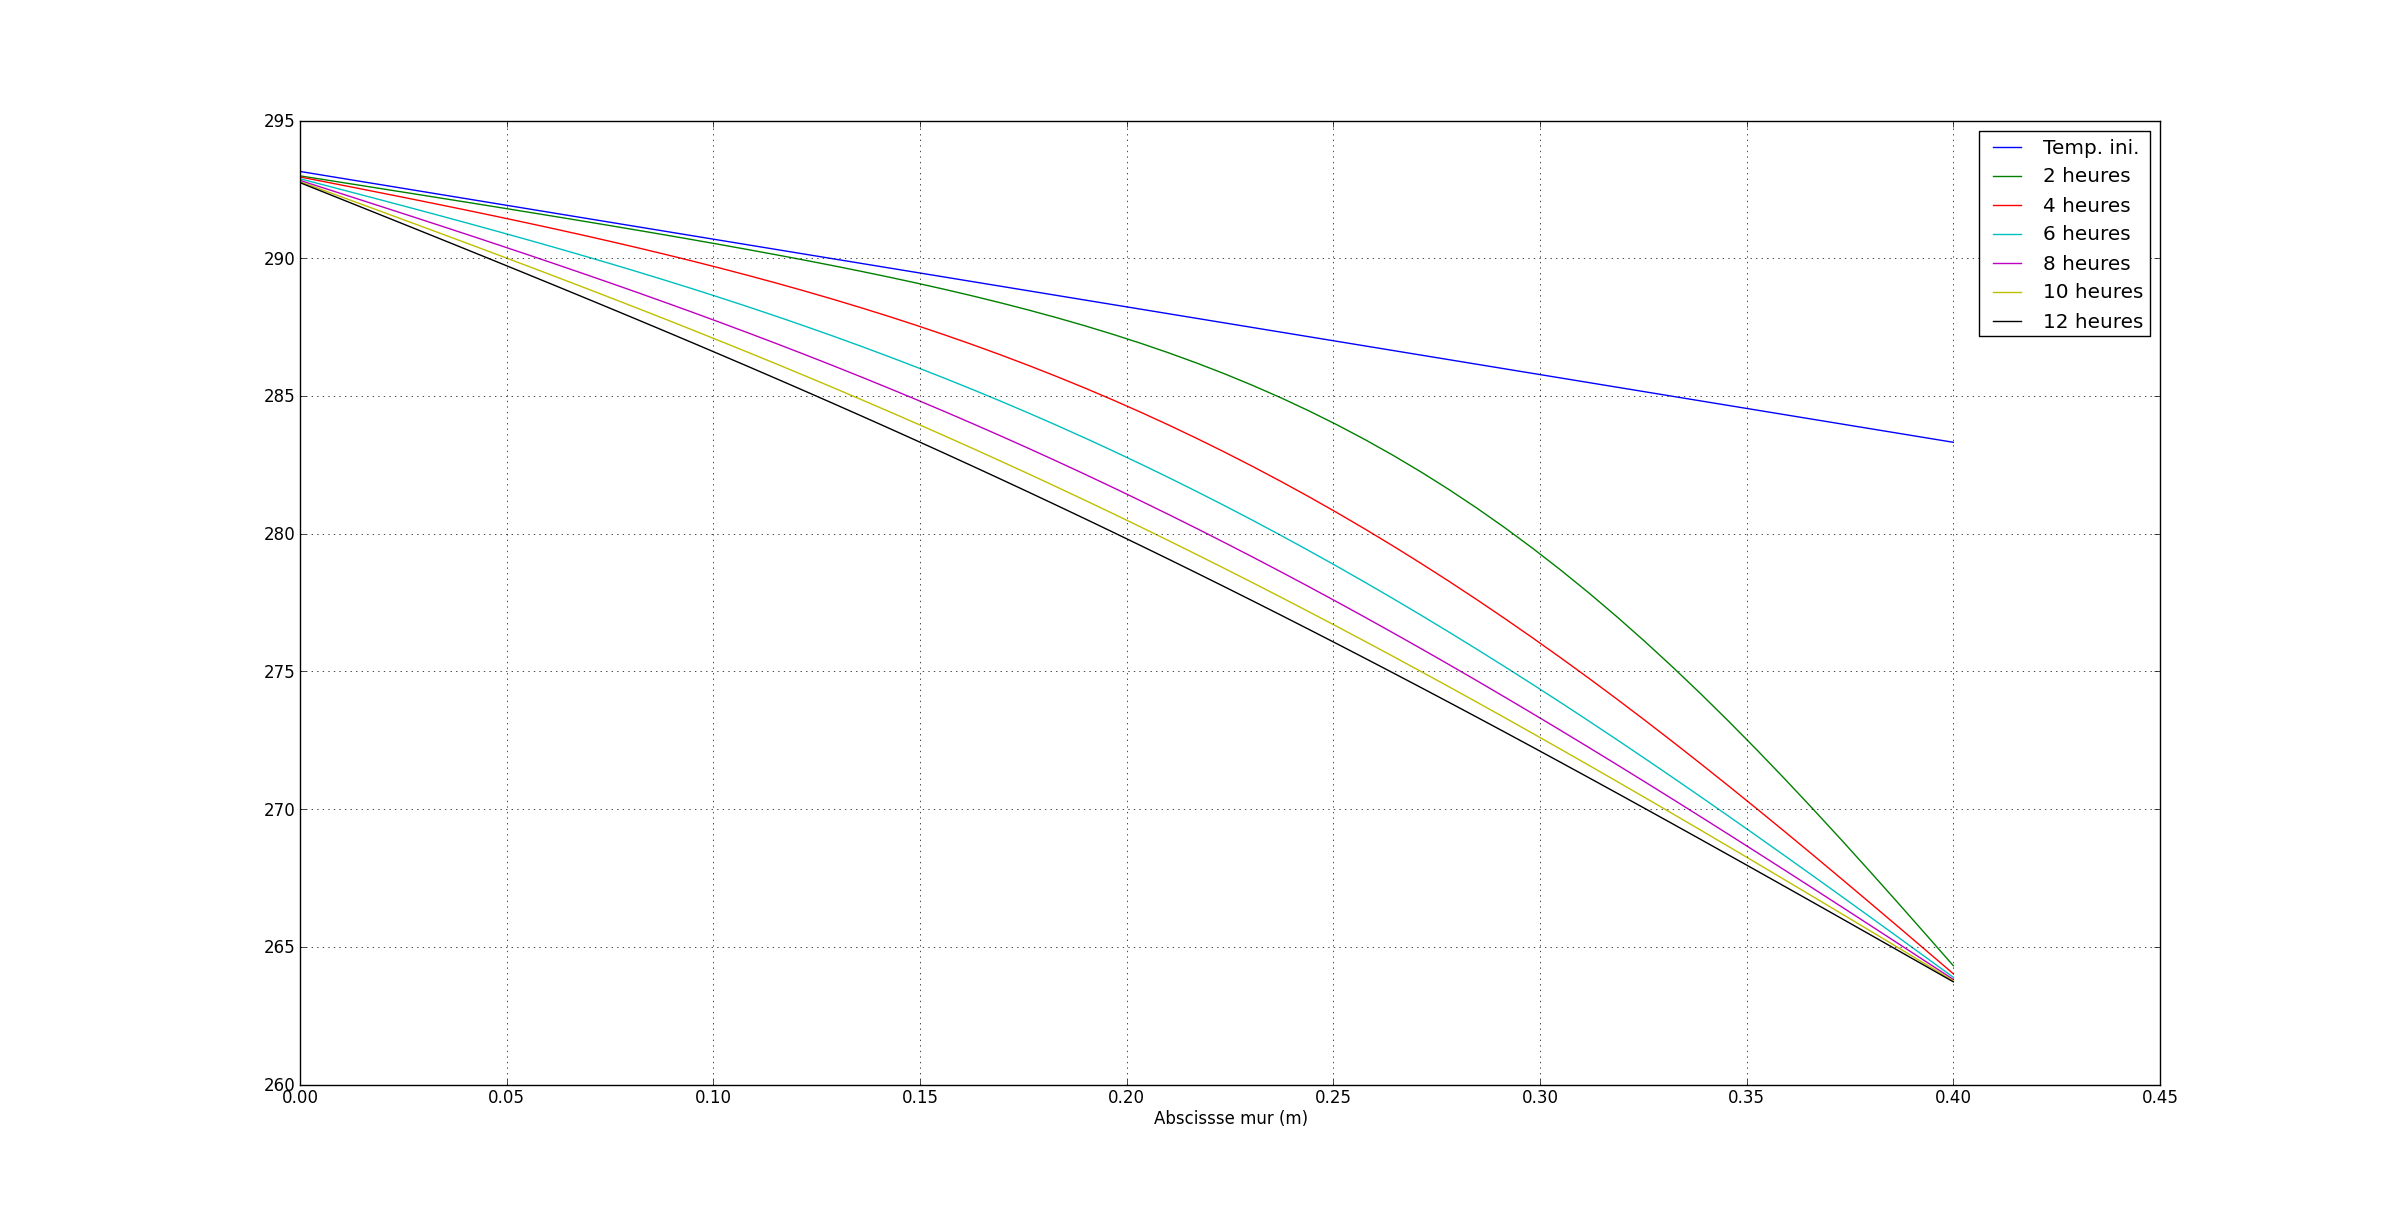
\includegraphics[width=\linewidth]{images/figure_04}
\end{center}


\subparagraph{}
\textit{Le pas de discrétisation temporel est de 30 secondes. Les résultats de la simulation sont stockés dans la 
matrice  \texttt{ T\_tous\_k}  définie précédemment. Écrire les instructions permettant de tracer le réseau de courbes 
précédentes.}

\vspace{.5cm}

Les résultats de la simulation sont codés dans un fichier texte codé en ASCII. L'écriture des nombres est limitée à 10 caractères (signe et virgule inclus). 
Le mur est discrétisé en 100 abscisses. Le pas de discrétisation temporel est de 30 secondes. 


\subparagraph{}
\textit{Quelle sera la taille du fichier texte généré ?}
\fi

\ifprof
\begin{corrige}
\question\
\begin{python}
k=[0,240,480,720,960,1200,1440]
les_X=[i*0.4/(N+1) for i in range(N+2)]
for i in k:
    plt.plot(les_X,T_tous_k[:,i])
plt.show()
\end{python}


\question\
Le régime permanent est atteint au bout de 12 heures. Avec un pas temporel de 30 secondes, il y a donc $12\times 120$ 
soit 2400 itérations. Si on considère que $Itmax=2400$, on aura donc $100 \times 2400$ valeurs. Pour l'estimation de la 
taille du fichier on fait ici l'abstraction du codage des espaces et des retours à la ligne. 
La taille du fichier est donc : $100 \times 2400 \times 10 \times 1 \simeq 2,4\, \text{Mo}$.
\end{corrige}
\else

\section{Annexe}
\noindent
Dans tout le problème, on suppose que la bibliothèque \textbf{Numpy} a été chargée.\\
Tous les vecteurs et matrices intervenant seront des tableaux de numpy (array).\\
Par exemple, on peut définir des vecteurs par :\\
 $U=array([1,2,3])$ et $V=array([1,0,1]]$.\\
On a comme pour des listes : $U[0]=1, U[1]=2, V[1]=0$...\\
On peut définir une matrice par $M=array([[1,1,2],[1,-1,0],[0,1,3]])$ c'est la matrice
 $M=\left(\begin{array}{ccc}1&1&2\\1&-1&0 \\ 0&1&3 \end{array} \right)$.\\
De même , par exemple, on a $M[0,2]=2$. \\
On peut additionner deux vecteurs : $U+V=array([2,2,4])$, multiplier par un scalaire :
$3*U=array([2,6,9])$ .\\
Pour effectuer le produit scalaire on fait \textbf{vdot(u,v)}.\\
Pour effectuer le calcul de $MU$ on fait \textbf{dot(M,U)}.\\
On peut aussi définir un vecteur de taille $N$ contenant des zéros par l'instruction 
$A=$\textbf{zeros([N])} et une matrice de taille $i\times j$ contenant des zéros par 
$M=$\textbf{zeros([i,j])} .
\fi


